\documentclass{vldb}
\usepackage{graphicx}
\usepackage{balance} 

\begin{document}


\section{Introduction}

\section{Problem Statement}
\subsection{Background}
Movie genres are manually created categorical labels to characterize different movies. These genre labels can be used to describe the movie, contribute in movie recommendation based on the domain specified interests and some other fields. Currently the movie genres annotation are determined by us. The complexity in automatic genre classification is caused by the fact that usually the genres are not well  defined. Normally there are no strict definitions or boundaries between 2 different genres.  And of cause they share certain overlapping characteristics.
\par Facing the fact that the number of movie is growing at a fast pace, automatic movie genres classification can assist or replace the human work in this process and provide important component for the complete movie information and in addition, structure the movie based on the genres. Thus, we begin to think about: what kind of information is sufficient to automatically classify the movie and how to approach that?
\par After considering our requirement and all the related movie information component, We decide to focus on building a scalable movie genre classification system based on their plot description. 

\subsection{Dataset} 
Dataset:The dataset we use is the publicly available data from the Internet Movie Database(IMDb). IMDb is an online dataset which provides information related to movies, television programs and video games. The information includes actors, production crew and fictional characters featured in these. There are some publicly available datasets containing a subset of the online database, which can be downloaded and processed. 
\par The dataset is organized into a set of compressed text files, where each file contains information on a specific aspect. The files we use are the plot.list and genres.list files and the size is more than 400MB. It contains all the plot description, genre information we need and is big enough to test the scalability.
\subsection{Tools}
\par Python: Python is a fast and friendly language. It’s easy to learn and can work everywhere. The raw data from IMDb can not be used directly, so we choose Python to do the preprocessing work and generate processed data for the next steps.
\par Apache Spark: Spark is an open source Apache project built around speed, ease of use. It provides a faster and more general data processing platform. Spark enables we to quickly write applications in Java, Scala, or Python. It comes with a built-in set of over 80 high-level operators. And we can use it interactively to query data within the shell. Other than Spark Core API, there are additional libraries that are part of the Spark ecosystem and provide additional capabilities in Big Data analytics and Machine Learning areas. The scalable machine learning library consisting of common learning algorithms and utilities, including classification, regression, clustering, collaborative filtering, dimensionality reduction, as well as underlying optimization primitives.

\section{Methodology}
\subsection{Apache Spark Pipeline}
In machine learning, it is common to run a sequence of algorithms to process and learn from the data, a regular text document processing workflow might include several steps like:
\begin{itemize}
\item {Split the document into words.}
\item {Convert each document's words into a numerical feature vector.}
\item {Learn a prediction model using the feature vectors and labels.}
\end{itemize}
\par Spark ML represents such a workflow as a Pipeline, which consists of a sequence of PipelineStages (each stage is either a Transformer or an Estimator) to be run in a specific order. The input dataset is modified as it passes through each stage. For Transformer stages, the transform() method is called on the dataset. For Estimator stages, the fit() method is called to produce a Transformer (which becomes part of the PipelineModel, or fitted Pipeline), and that Transformer’s transform() method is called on the dataset.
\par This figure shows the 3-stage pipeline we used in the project. These 3 stages are all transformers.  Each stage’s transform() method updates the dataset and passes it to the next stage. The bottom row represents data flowing through the pipeline, where cylinders indicate DataFrames. The Tokenizer.transform() method splits the raw text documents into words, adding a new column with words into the dataset. The HashingTF.transform() and idf.transform() method converts the words column into feature vectors, adding a new column with those vectors to the dataset. Then SVM.train() is called to produce a SVMModel. After that the pipeline calls SVM.predict() method on the dataset and predict the result.
\begin{figure}
\begin{center}
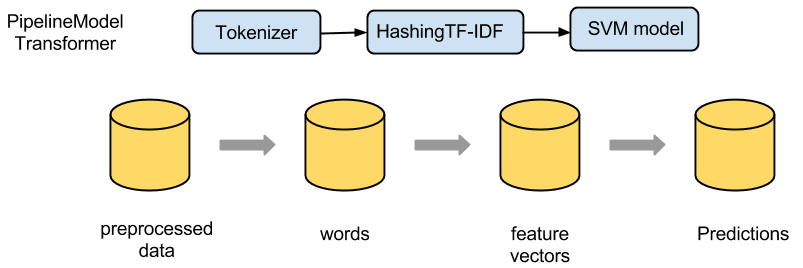
\includegraphics[width=3.50in]{AIM3-pipeline.png}
\caption{movie genres classification pipeline}
\end{center}
\end{figure}
\subsection{Preprocessing}
\par To get start, we first use Tableau to get a insight of the dataset. 
\begin{figure}
\begin{center}
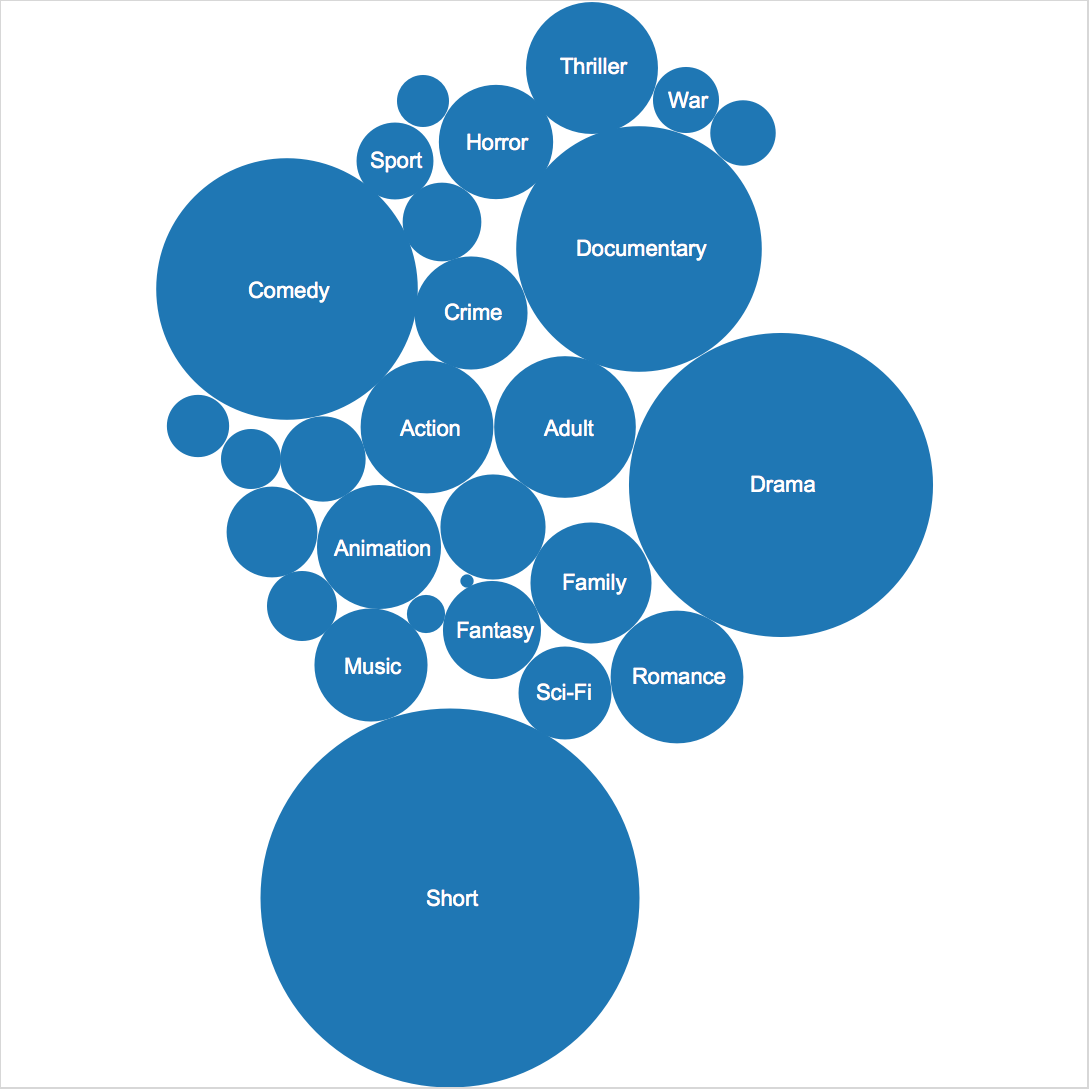
\includegraphics[width=3.00in]{tableau.png}
\caption{insight of the data using Tableau}
\end{center}
\end{figure}
\subsection{Feature Extraction}
Term frequency-inverse document frequency (TF-IDF) is a feature vectorization method that is intended to reflect how important a word is to a document in a collection of the corpus. The tf-idf value increases probability to the number of times a word appears in the document, but is offset by the frequency of the word in the corpus, which helps to adjust for the fact that some words appear more frequently in general.
\par Denote a term by $t$, a document by $d$, and the corpus by $D$. Term frequency $TF(t,d)$ is the number of times term $t$ appears in document $d$, while the document frequency $DF(t,D)$ is the number of documents that contain term $t$ in corpus $D$. However, if we only use term frequency, for some common words, like "the", it will tend to incorrectly emphasize the documents which happen to use "the" more frequently. But these kind of words can't provide enough information to distinguish relevant and non-relevant documents and terms. If a term appears very often across the corpus, it means it doesn’t carry special information about a particular document. Thus, we use inverse document frequency, a numerical measure to show how much information a term carries:
\begin{displaymath}
IDF(t,D) = \log\frac{|D|+1}{DF(t,D)+1},
\end{displaymath}
where $|D|$ is the number of documents in the corpus. Since logarithm is used, if a term appears in all documents, its $IDF$ value becomes 0. Note that a smoothing term is applied to avoid dividing by zero for terms outside the corpus. The TF-IDF measure is simply the product of $TF$ and $IDF$:
\begin{displaymath}
TFIDF(t,d,D)=TF(t,d)⋅IDF(t,D).
\end{displaymath} 
\par Also, in the implementation of TF-IDF of in  Apache Spark machine learning library, raw feature is mapped into an index(term) by using a hashing function. Then term frequency is calculated based on the mapped indices. This approach avoids the need to compute a global term-to-index map, which can be expensive for a large corpus, but it suffers from potential hash collisions, where different raw features may become the same term after hashing. To reduce the chance of collision, we can increase the target feature dimension, i.e., the number of buckets of the hash table. The default feature dimension is $2^{20}=1048576$
\par By using tf-idf, we generate a vector for every plot description.

\subsection{Classification}
In machine learning, support vector machines(SVMs) are supervised learning models used for classification and regression analysis. Given a set of training examples, each marked for belonging to one of two categories, an SVM training algorithm builds a model that assigns new examples into one category or the other, making it a non-probabilistic binary linear classifier. 
\par An SVM model constructs a hyperplane in high(or infinite)dimensional space, which can be used for classification, regression, or other tasks. Intuitively, a good separation is achieved by the hyperplane that has the largest distance to the nearest training-data point of any class (so-called functional margin), since in general the larger the margin the lower the generalization error of the classifier.
\par Given some training dataset $\mathcal{D}$ containing $n$ points:
\begin{displaymath}
\mathcal{D} = \{(\mathbf{x}_i,y_i)|\mathbf{x}_i \in \mathbb{R}^p,y_i\in\{-1,1\}\}^n _{i=1}
\end{displaymath}
where $y_i$ is either $1$ or $-1$, indicating the class to which $\mathbf{x}_i$ belongs. Each $\mathbf{x}_i$ is a $p$ dimentional vector. If the data is linealy seperable, we can find a hyperplane:
\begin{displaymath}
\mathbf{w}\cdot\mathbf{x}-b=0 
\end{displaymath}
to seperate the dataset and by determin the distance from the data point to the hyperplane $|\mathbf{w}\cdot\mathbf{x}+b|$ is positive or negative to see which class this pint belongs to.

\par  To find the maximum margin to divide the dataset into 2 classes($y=1$ or $y=-1$), we can select two hyperplanes in a way that they separate the data and there are no points between them, and then try to maximize their distance. The region bounded by them is called "the margin". These hyperplanes can be described by the equations
\begin{displaymath}
\mathbf{w}\cdot\mathbf{x}-b=1
\end{displaymath}
and
\begin{displaymath}
\mathbf{w}\cdot\mathbf{x}-b=-1
\end{displaymath}
\begin{figure}
\begin{center}
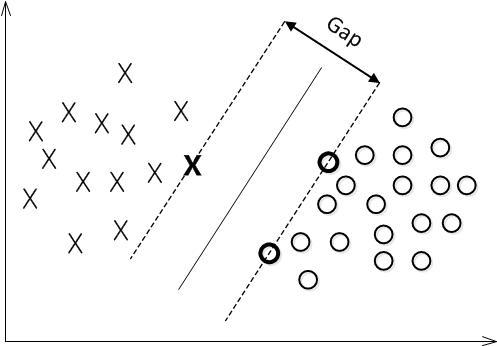
\includegraphics[width=2.50in]{SVM.jpeg}
\caption{margins for an SVM trained with samples from two classes}
\end{center}
\end{figure}
\par By using geometry, we find the distance between these two hyperplanes is $\frac{2}{||w||}$, so we want to minimize $||w||$. As we also have to prevent data points from falling into the margin, we add the following constraint:
\begin{displaymath}
\begin{cases}
\mathbf{w}\cdot\mathbf{x}-b\ge1,y_i=1\\
\mathbf{w}\cdot\mathbf{x}-b\le-1,y_1=-1\\
\end{cases}
\end{displaymath}
This can be written as:
\begin{displaymath}
y_i(\mathbf{w}\cdot\mathbf{x}_i-b)\ge1,1\le i \le n
\end{displaymath}
\par More clearly, the constraint problem can be written as:
\begin{displaymath}
\arg\min\frac{1}{2}||\mathbf{w}||^2
\end{displaymath}
subject to (for any $i = 1,...,n$)
\begin{displaymath}
y_i(\mathbf{w}\cdot\mathbf{x}_i-b)\ge1
\end{displaymath}
After getting the $\mathbf{w}$, given a new data point, denoted by $\mathbf{x}$
\section{Experiment}
\section{Results}
\section{Conclution}
\section{Reference}


\end{document}
